\chapter{Wprowadzenie teoretyczne}\label{chapter2}

W niniejszym rozdziale przedstawiono podstawowe pojęcia związane z dziedziną muzyki, syntezy dźwięku oraz przetwarzania sygnałów cyfrowych. Omówione zagadnienia odnoszą się do całości pracy, nie są one powiązane szczególnie z konkretnymi metodami syntezy. Przedstawienie ich w początkowej części pracy ma na celu ułatwienie czytelnikowi zrozumienia dalszej części pracy.



\section{Dźwięk}
Dźwięk można rozpatrywać na dwa sposoby: fizyczny oraz muzyczny. Z fizycznego punktu widzenia, dźwięk jest zaburzeniem falowym w ośrodku sprężystym gazowym, ciekłym lub stałym, który wywołuje wrażenie słuchowe u człowieka. Poddziedzina fizyki, zajmująca się ściśle tematem dźwięku, nazywana jest akustyką.
% (źródło: https://encyklopedia.pwn.pl/haslo/dzwiek;3896050.html) 

W muzyce, dźwięk rozpatrywany jest jako zjawisko, które wydobywane jest z instrumentów muzycznych lub głosu ludzkiego. Główne właściwości dźwięku w muzyce, to:

\begin{enumerate}
	\item wysokość dźwięku, która jest zależna od wartości częstotliwości podstawowej dźwięku,
	
	\item czas trwania - zależny od czasu produkowanego dźwięku na danym instrumencie,
	
	\item głośność, zależna od amplitudy drgań powietrza przenoszącego dźwięk, mierzona w decybelach,
	
	\item barwa dźwięku, zależna od ilości, częstotliwości składowych harmonicznych dźwięku oraz zmian ich występowania w czasie. Jako składowa harmoniczna, rozumiana jest składowa sinusoidalna dźwięku, która jest całkowitą wielkrotnością częstotliwości podstawowej danego dźwięku.
	% (źródło: https://pl.wikipedia.org/wiki/D%C5%BAwi%C4%99k_(muzyka))
\end{enumerate}

Jako pewne ustandardyzowanie dźwięków w utworach muzycznych, wprowadzono skalę dźwięków. Tradycyjną skalę tworzy osiem dźwięków. Odległości między tymi dźwiękami nazywane są interwałami, które wyraża się w jednostkach półtonów. Istnieje zależność między kolejnymi półtonami i może być ona wyrażona wzorem:
\begin{equation} \label{equ:idft}
k = f(\sqrt[12]{2})^{n}
\end{equation}
\begin{tabular}{ l l l l}
	gdzie: 	&	$f$ & - &  częstotliwość tonu dźwięku, od którego liczona jest odległość, \\
	&	$k$ & - &  częstotliwość tonu, do którego liczona jest odległość, \\
	&   $n$ &  - & odległość tonu o częstotliwości f od tonu o częstotliwości k w półtonach, \\
\end{tabular}

Odstęp między pierwszym a ostatnim dźwiękiem w skali nazywany jest oktawą. Mierzy on 12 półtonów. Odległość ta jest wyjątkowa, gdyż dźwięk położony o oktawę dalej od pierwszego, jest jego dwukrotnością pod względem częstotliwości podstawowej składowej harmonicznej.



\section{Rodzaje klawiatur muzycznych}
Podstawowy podział klawiatur muzycznych rozpatruje się pod względem możliwości wydawania z siebie jednego lub kilku dźwięków przy naciśnięciu kilku klawiszy na raz. Typy te nazwano klawiaturami monofonicznymi oraz polifonicznymi.

\subsection{Klawiatura monofoniczna}
Monofonia w muzyce to faktura muzyczna utworzona z pojedynczej linii melodycznej. W danej chwili czasu utworu, powinien występować tylko jeden dźwięk, aby był on nazwany monofonicznym. W szczególnym odniesieniu do klawiatury cyfrowej lub analogowej oznacza to, iż wydobywać się z niej może się maksymalnie jeden dźwięk w jednym momencie czasu, przy naciśnięciu kilku klawiszy. Klasycznym przykładem klawiatury monofonicznej jest syntezator analogowy Minimoog.

\subsection{Klawiatura polifoniczna}
Polifonia w muzyce oznacza natomiast występowanie kilku linii melodycznych w tym samym czasie. Polifonia klawiatury zatem oznacza możliwość wydobycia wielu dźwięków, przy naciśnięciu kilku klawiszy w tym samym czasie. Pojęcie polifonicznej klawiatury muzycznej nie precyzuje ilości wydobywających się dźwięków jaką klawiatura powinna móc realizować. Cyfrowe instrumenty muzyczne na rynku posiadają ograniczoną maksymalną liczbę wydobywanych na raz dźwięków, przez skończoną moc obliczeniową procesorów.

%
% Voice allocation alghorithm - opisac jaki bedziemy uzywac
%

Jednym z głównych zadań niniejszego projektu magisterskiego jest implementacja polifonicznej klawiatury muzycznej.



\section{Przegląd metod syntezy dźwięku}
% http://legacy.spa.aalto.fi/publications/reports/sound_synth_report.pdf
Podział metod syntezy dźwięku w literaturze jest bardzo zróżnicowany. Najczęściej spotykany podział występuje pod względem różnych podejść do syntezy:
\begin{enumerate}
	\item metody widmowe,
	\item algorytmy abstrakcyjne,
	\item metody fizyczne,
	\item metody przetwarzania sygnału,
	% https://ieeexplore.ieee.org/document/4412805
\end{enumerate}

W poniższych podrozdziałach scharakteryzowano poszczególne rodzaje metod syntezy dźwięku.

\subsection{Metody widmowe}
Do grupy widmowych metod syntezy dźwięku zaliczana jest synteza subtraktywna oraz addytywna. Zgodnie z nazwą, skupiają się one na syntezie brzmień w dziedzinie częstotliwości. Metoda subtraktywna zajmuje się głównie wycinaniem pasm widmowych z brzmień obfitych w składowe harmoniczne. Metoda addytywna skupia się natomiast na dodawaniu kolejnych harmonicznych w dziedzinie częstotliwości. Obie metody zostały dokładnie omówione w kolejnych rozdziałach [jakie rozdziały? - zrobic odnosnik] niniejszej pracy.

\subsection{Algorytmy abstrakcyjne}
% https://ccrma.stanford.edu/~bilbao/booktop/node6.html
% http://legacy.spa.aalto.fi/publications/reports/sound_synth_report.pdf
Synteza poprzez algorytmy abstrakcyjne zazwyczaj odnosi się do zmian istniejących już dźwięków poprzez filtry nieliniowe lub funkcje matematyczne. Do metod algorytmów abstrakcyjnych należą między innymi synteza FM, synteza AM, synteza poprzez waveshaping lub algorytm Karplus-Strong. W literaturze można również spotkać się z określaniem tej grupy metod syntezy jako Distortion synthesis (synteza poprzez zakłócanie), która odnosi się do wprowadzanych zmian w istniejącym już dźwięku (zakłóceń). W niniejszej pracy poświęcono cały rozdział dla pierwszej z wymienionych metod - syntezy FM.

\subsection{Metody fizyczne}
% https://ccrma.stanford.edu/~bilbao/booktop/node12.html
% https://edu.pjwstk.edu.pl/wyklady/mul/scb/main37.html
Metody fizyczne skupiają się na odwzorowywaniu instrumentów muzycznych poprzez tworzenie ich modeli fizycznych na różne sposoby. Do tej grupy należą synteza poprzez modelowanie matematyczne, synteza komórkowa (ang. Cellular Sound Synthesis) oraz synteza falowodowa (ang. Digital Waveguide Modeling).

Metody syntezy oparte na modelach fizycznych są uważane za najbardziej naukowe i poświęcone jest im wiele prac naukowych. W niniejszej pracy, z tej grupy metod syntezy, przedstawiono głównie synteze fizyczną opartą o modelowanie matematyczne.

\subsection{Metody przetwarzania sygnału}
%http://marcdata.hamu.cz/vyzkum/dokumenty/Lit92.pdf - additive, subtractive, FM. sampling
%https://soundlab.cs.princeton.edu/publications/survey_icmc09.pdf - 4 strona, tabelka
%https://www.youtube.com/watch?v=I64y40EIPaM
Jako metody przetwarzania sygnału rozumiane są takie metody syntezy, które oddziaływują bezpośrednio na próbkach sygnału cyfrowego. Do tej grupy metod należą między innymi synteza tablicowa (wavetable), synteza granularna oraz synteza poprzez samplowanie.

Synteza poprzez samplowanie jest najbardziej powszechną metodą syntezy dźwięku w tej grupie. Polega ona na użyciu fragmentu wcześniej dokonanego nagrania (sampla) i odtwarzanie go dla różnych wysokości dźwięków. Jest to metoda najczęściej używana przez kompozytorów w dzisiejszych czasach.

Z uwagi na nieunaukowy charakter tego rodzaju syntezy dźwięku, żadna synteza należąca do tej grupy nie została opisana w tej pracy.



\section{Klasyczne moduły syntezatorów dźwięku}
%https://www.dummies.com/art-center/music/piano/common-keyboard-terms-and-abbreviations/
%https://en.wikipedia.org/wiki/Modular_synthesizer#:~:text=Modular%20synthesizers%20are%20synthesizers%20composed,user%20to%20create%20a%20patch.
Syntezatory analogowe są nazywane również modularnymi ze względu na ich budowę. Utworzenie dźwięku przez taki syntezator wymaga przejścia drogi od źródła, którym jest zazwyczaj pewien oscylator lub generator szumu, przez odpowiednie filtry, do wyjścia.

\begin{figure}[H]
	\centering
	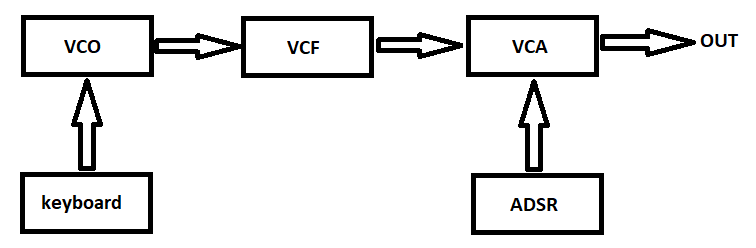
\includegraphics[width=12cm]{./grafiki/analog_synth_scheme}
	\captionsetup{justification=centering}
	\caption{Schemat podstawowego syntezatora modularnego (analogowego).}
	\label{rys:analog_scheme}
\end{figure}

Na rysunku \ref{rys:analog_scheme} przedstawiono podstawowy schemat syntezatora modularnego. Składa się on z najbardziej powszechnych modułów, stosowanych w analogowej syntezie dźwięku. Przebieg tworzony jest przez oscylator (VCO), którego częstotliwość zostaje narzucona przez naciśnięcie klawisza o odpowiedniej wysokości dźwięku. Następnie dźwięk trafia na filtr (VCF) i zostaje pozbawiony pewnej części składowych harmonicznych. W dalszej kolejności dociera on na moduł sterujący amplitudą dźwięku (VCA), który ustawia jego amplitudę zgodnie z ustawieniami modułu ADSR. Następnie dźwięk trafia na wyjście, czyli na urządzenie nagłaśniające.

W cyfrowej syntezie dźwięku, każdy z tych modułów jest realizowany jako część programu na procesorze klasy DSP. Poniżej opisano bardziej szczegółowo moduły, które będą realizowane jako część programu w ramach tej pracy.

\subsection{ADSR}
Akronim, który jest tytułem tego podrozdziału, oznacza cztero-etapowy generator obwiedni stosowany w syntezatorach. Jest on wykorzystywany zarówno w syntezatorach analogowych, jak i cyfrowych.

% źródło: D:/Data/Studia/Magisterka/Literatura%20wstepna/synthesizers__a_brief_introduction.pdf
\begin{figure}[H]
	\centering
	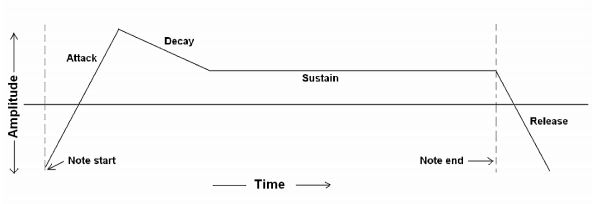
\includegraphics[width=15cm]{./grafiki/ADSR}
	\captionsetup{justification=centering}
	\caption{Generator obwiedni dźwięku (ADSR).}
	\label{rys:ADSR}
\end{figure}

Na rysunku \ref{rys:ADSR} przedstawiono przykładową obwiednie dźwięku po naciśnięciu klawisza. Poniżej wytłumaczone zostały kolejne etapy ADSR:
\begin{enumerate}
	\item Attack - czas narastania amplitudy od zera to maksimum, rozpoczyna się, gdy klawisz zostaje naciśnięty,
	
	\item Decay - czas opadania amplitudy od maksymalnej wartości do poziomu podtrzymania,
	
	\item Sustain - poziom amplitudy przy podtrzymaniu dźwięku, trwa dopóki klawisz nie zostanie puszczony,
	
	\item Release - czas opadania amplitudy dźwięku od poziomu wyznaczonego przez Sustain do zera.
\end{enumerate}


\section{Analogowa i cyfrowa synteza dźwięku}
% Porownanie: https://www.synthtopia.com/content/2019/01/11/analog-vs-digital-synthesizer-blind-test/  W opisie na YT sa wyniki
Debata na temat tego, który rodzaj syntezatorów jest lepszy, trwa już od samego wprowadzenia syntezatorów cyfrowych na rynek. Argumenty za i przeciw obu stron tego konfliku zazwyczaj odnoszą się do charakteru brzmienia obu rodzajów syntezatorów. 

Lorenzo Furlanetto w ramach swojej pracy magisterskiej dokonał ślepego porównania klasycznego syntezatora analogowego oraz jego cyfrowej emulacji. Wyniki ślepego testu pokazały, iż 51 procent ankietowanych rozpoznało, który z syntezatorów był analogowy, natomiast aż 57 procent osób orzekło, iż dźwięk syntezatorów cyfrowych jest przyjemniejszy. Oznacza to, że ciężkim jest dokonanie odróżnienia syntezatorów cyfrowych od analogowych, oraz że większość ludzi preferuje brzmienie syntezatorów cyfrowych.

% https://blog.andertons.co.uk/labs/hardware-synths-vs-software-synths
Syntezatory cyfrowe, w stosunku do analogowych, posiadają wiele zalet. W tych pierwszych można dokonać syntezy wielu rodzajów dźwięków, w tym takich, które imitują brzmienie prawdziwych instrumentów. Syntezatory analogowe natomiast, pozwalają jedynie na uzyskanie prostych brzmień, przy pomocy filtracji i zmian podstawowych przebiegów. Dodatkowo, dzięki cyfrowemu łączeniu wielu maszyn cyfrowych, można sterować wieloma syntezatorami, za pomocą jednej klawiatury.

Z technicznego punktu widzenia, cyfrowe syntezatory są również lepsze z uwagi na ich cyfrowe przetwarzanie sygnałów. Filtry i inne elementy ciągu przetwarzania sygnału nie ulegają degradacji z czasem, z uwagi, iż są elementami programu na procesorze. Elementy analogowe należy wymieniać lub dostrajać. Dodatkowo, dzięki dużej szybkości próbkowania oraz taktowania procesorów, można uzyskać porządane charakterystyki. Częstotliwościowe obwiednie filtrów mogą być idealne, bez zbędnego pasma przejściowego.
% cos jeszcze?


\section{MIDI}
Cyfrowy interfejs instrumentów muzycznych (MIDI) to standard utworzony w 1983 roku, służący do przekazywania informacji między cyfrowymi instrumentami muzycznymi. Zrewolucjonizował on sektor muzyki elektronicznej. Dzięki wdrożeniu tego protokołu, muzycy mogli na scenie używać jednej klawiatury muzycznej podłączonej do wielu modułów dźwiękowych, zamiast posiadania tak zwanej "ściany syntezatorów". MIDI zawiera zarówno standard warstwy sprzętowej jak i zestaw komend służących do komunikacji urządzeń.

\subsection{Warstwa sprzętowa MIDI}
W interfejsie MIDI, informacje przesyłane są za pomocą szeregowego połączenia dwóch urządzeń cyfrowych, w trybie półdupleks. Szybkość przesyłu informacji została ustandardyzowana i wynosi 31250 bitów na sekundę. Podobnie jak w popularnym interfejsie UART, początek transmisji ramki danych rozpoczyna bit startu o wartości 0, natomiast kończy bit stopu o wartości logicznej jedynki. Interfejs MIDI jest interfejsem prądowym, gdzie logiczne zero oznacza brak przepływu prądu, natomiast logiczna jedynka oznacza jego przepływ.

\begin{figure}[H]
	\centering
	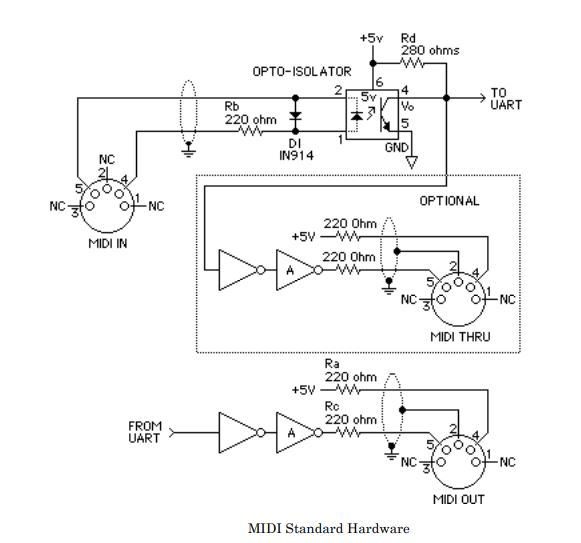
\includegraphics[width=9cm]{./grafiki/hardware_midi}
	\captionsetup{justification=centering}
	\caption{Schemat elektryczny interfejsu MIDI.}
	\label{rys:hardware_midi}
\end{figure}

Schemat sprzętowy interfejsu MIDI znajdującego się po stronie instrumentu cyfrowego przedstawiono na rysunku \ref{rys:hardware_midi}. Do połączeń z instrumentem używane są wtyki DIN pięciopinowe. Na wejściu interfejsu MIDI zawsze umieszczony zostaje transoptor, który chroni instrument dostający informację przed uszkodzeniem.

\subsection{Protokół MIDI}
%https://www.midi.org/specifications-old/category/midi-1-0-detailed-specifications
%PDF: D:\Data\Studia\Magisterka\Literatura wstepna\MIDI
Wiadomości MIDI utworzone są z jednego bajta statusu, po którym następuje zazwyczaj jeden lub dwa bajty danych. Są różne typy wiadomości MIDI. Najbardziej podstawowy podział dzieli je na wiadomości kanałowe (odnoszące się do jednego kanału) oraz systemowe (odnoszące się do wszystkich kanałów). Wiadomości kanałowe mogą dzielić się dalej na komunikaty trybu lub komunikaty głosu. Te drugie w praktyce stanowią większość przesyłanych komunikatów w transmisji MIDI.
Komunikat głosu może nieść informację na przykład o: naciśnięciu klawisza, odciśnięciu klawisza, aftertouch (zmiana mocy nacisku klawisza po jakimś czasie od naciśnięcia), pitch bend (delikatna zmiana wysokości dźwięku). Protokół MIDI, w ramach bajta danych (komunikat głosu), może obsłużyć 128 wysokości dźwięków z jednego instrumentu. Poziom głośności, zależny od mocy naciśnięcia klawisza, również może przyjąć jedną ze 128 wartości.

Poza całym przesyłam informacji między dwoma urządzeniami MIDI, występuje dodatkowo zegar MIDI (ang. MIDI Pulses), który pozwala na zsynchronizowanie dwóch instrumentów, aby grały w jednakowym tempie. Wiadomości występują cyklicznie i zawsze posiadają tę samą wartość bitową.



\section{Dyskretna transformacja Fouriera}
%Technika cyfrowego przetwarzania sygnałów - A. Leśnicki
Jednym z najważniejszych narzędzi w dziedzinie cyfrowego przetwarzania sygnałów jest dyskretna transformata Fouriera (DFT). Jest to przekształcenie zdefiniowane dla skończonych sygnałów dyskretnych. Pozwala ono na transformację dyskretnego sygnału czasowego na próbki widma dyskretnego. Posiada ono również swój odpowiednik zwany IDFT, który pozwala na przekształcenie dyskretne odwrotne, z widma do sygnału czasowego.

\subsection{Definicja przekształcenia DFT}
%Technika cyfrowego przetwarzania sygnałów 262 strona - A. Leśnicki
Dyskretne przekształcenie Fouriera oraz odwrócone dyskretne przekształcenie Fouriera są kolejno przedstawione następującymi wzorami:
\begin{equation} \label{equ:dft}
X[k] = \sum_{n=0}^{N-1} x[n]e^{-j\frac{2\pi k}{N}n}
\end{equation}
\begin{equation} \label{equ:idft}
x[n] = \frac{1}{N}\sum_{k=0}^{N-1} X[k]e^{j\frac{2\pi n}{N}k}
\end{equation}
\begin{tabular}{ l l l l}
	gdzie: & $X[k]$ &  - & k-ta próbka widma dyskretnego sygnału, \\
	&	$x[n]$ & - &  n-ta próbka dyskretnego sygnału w dziedzinie czasu, \\
	&	$N$ & - &  ilość próbek sygnału poddanego przekształceniu Fouriera,\\
	&	$n$ & = &  próbki dyskretnego sygnału, n = 0, 1, 2, ..., N - 1 \\
\end{tabular}

We wzorach \ref{equ:dft} i \ref{equ:idft} przyjęto indeksowanie asymetryczne.

\subsection{Algorytm FFT}
%Technika cyfrowego przetwarzania sygnałów 292 strona - A. Leśnicki
Wyznaczenie widma dyskretnego bezpośrednio z definicji \ref{equ:dft} jest bardzo wymagające obliczeniowo. Przy założeniu, że próbki sygnału poddanego przekształceniu są liczbami zespolonymi, do obliczenia DFT wymagane jest $N^{2}$ mnożeń zespolonych oraz $N(N-1)$ dodawań zespolonych.

W praktyce obliczenia DFT sygnału wykonuje się z wykorzystaniem bardzo efektywnego algorytmu szybkiej transformacji Fouriera (FFT, ang. Fast Fourier Transform). Algorytm został przedstawiony w 1965 roku i zapoczątkował nowy rozdział w dziedzinie cyfrowego przetwarzania sygnałów. Złożoność obliczeniowa tego algorytmu wynosi $\frac{N}{2}log_{2}N$. Algorytm FFT można stosować również do obliczenia transformacji odwrotnej IDFT.

%https://en.wikipedia.org/wiki/File:DIT-FFT-butterfly.png
%https://pl.qwe.wiki/wiki/Butterfly_diagram
\begin{figure}[H]
	\centering
	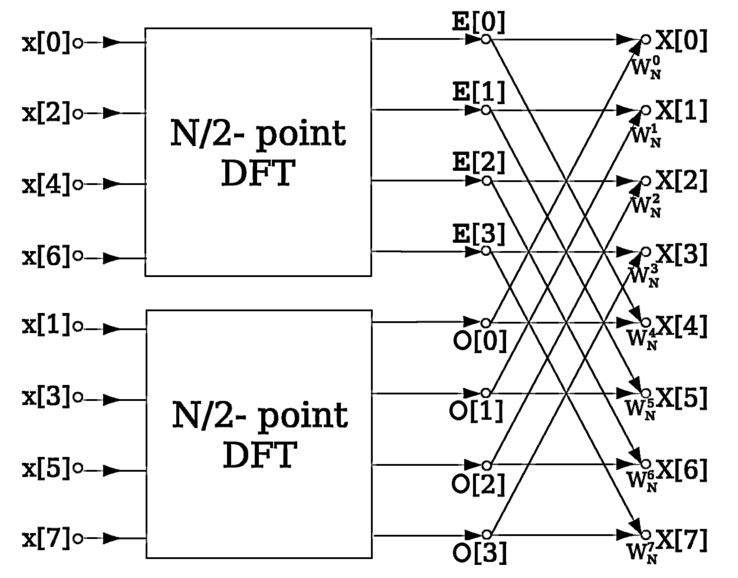
\includegraphics[width=10cm]{./grafiki/fft_motylki}
	\captionsetup{justification=centering}
	\caption{Algorytm FFT - schemat motylkowy.}
	\label{rys:fft_motyl}
\end{figure}

Działanie algorytmu dla sygnału 8-próbkowego przedstawione zostało na schemacie \ref{rys:fft_motyl}.